\documentclass[author-year, review]{elsarticle} %review=doublespace preprint=single 5p=2 column
%\documentclass[author-year, review]{elsarticle} %review=doublespace preprint=single 5p=2 column
%%% Begin My package additions %%%%%%%%%%%%%%%%%%%
\usepackage[hyphens]{url}
\usepackage{lineno} % add 
%\linenumbers % turns line numbering on 
\bibliographystyle{elsarticle-harv}
\biboptions{sort&compress} % For natbib
\usepackage{graphicx}
\usepackage{booktabs} % book-quality tables
%% Redefines the elsarticle footer
\makeatletter
\def\ps@pprintTitle{%
 \let\@oddhead\@empty
 \let\@evenhead\@empty
 \def\@oddfoot{\it \hfill\today}%
 \let\@evenfoot\@oddfoot}
\makeatother

% A modified page layout
\textwidth 6.75in
\oddsidemargin -0.15in
\evensidemargin -0.15in
\textheight 9in
\topmargin -0.5in
%%%%%%%%%%%%%%%% end my additions to header



\usepackage[T1]{fontenc}
\usepackage{lmodern}
\usepackage{amssymb,amsmath}
\usepackage{ifxetex,ifluatex}
\usepackage{fixltx2e} % provides \textsubscript
% use upquote if available, for straight quotes in verbatim environments
\IfFileExists{upquote.sty}{\usepackage{upquote}}{}
\ifnum 0\ifxetex 1\fi\ifluatex 1\fi=0 % if pdftex
  \usepackage[utf8]{inputenc}
\else % if luatex or xelatex
  \usepackage{fontspec}
  \ifxetex
    \usepackage{xltxtra,xunicode}
  \fi
  \defaultfontfeatures{Mapping=tex-text,Scale=MatchLowercase}
  \newcommand{\euro}{€}
\fi
% use microtype if available
\IfFileExists{microtype.sty}{\usepackage{microtype}}{}
\usepackage{graphicx}
% We will generate all images so they have a width \maxwidth. This means
% that they will get their normal width if they fit onto the page, but
% are scaled down if they would overflow the margins.
\makeatletter
\def\maxwidth{\ifdim\Gin@nat@width>\linewidth\linewidth
\else\Gin@nat@width\fi}
\makeatother
\let\Oldincludegraphics\includegraphics
\renewcommand{\includegraphics}[1]{\Oldincludegraphics[width=\maxwidth]{#1}}
\ifxetex
  \usepackage[setpagesize=false, % page size defined by xetex
              unicode=false, % unicode breaks when used with xetex
              xetex]{hyperref}
\else
  \usepackage[unicode=true]{hyperref}
\fi
\hypersetup{breaklinks=true,
            bookmarks=true,
            pdfauthor={},
            pdftitle={Early warning signals: The charted and uncharted territories},
            colorlinks=true,
            urlcolor=blue,
            linkcolor=magenta,
            pdfborder={0 0 0}}
\urlstyle{same}  % don't use monospace font for urls
\setlength{\parindent}{0pt}
\setlength{\parskip}{6pt plus 2pt minus 1pt}
\setlength{\emergencystretch}{3em}  % prevent overfull lines
\setcounter{secnumdepth}{0}
% Pandoc toggle for numbering sections (defaults to be off)
\setcounter{secnumdepth}{0}
% Pandoc header



\begin{document}
\begin{frontmatter}
  \title{Early warning signals: The charted and uncharted territories}
  \author[cstar]{Carl Boettiger\corref{cor1}}
  \ead{cboettig@gmail.com}
  \author[esp]{Noam Ross\corref{cor1}}
  \ead{noam.ross@gmail.com}
  \author[esp]{Alan Hastings}
  \cortext[cor1]{authors contributed equally}
  \address[cstar]{Center for Stock Assessment Research, Department of Applied Math and Statistics, University of California, Mail Stop SOE-2, Santa Cruz, CA 95064, USA}
  \address[esp]{Department of Environmental Science and Policy, University of California Davis, 1 Shields Avenue, Davis, CA 95616 USA}

  \begin{abstract}

The realization that complex systems such as ecological communities can collapse or shift regimes suddenly and without rapid external forcing poses a serious challenge to our understanding and management of the natural world.  The potential to identify early warning signals that would allow researchers and managers to predict such events before they happen has therefore been an invaluable discovery that offers a way forward in spite of such seemingly unpredictable behavior.  Research into early warning signals has demonstrated that it is possible to define and detect such early warning signals in advance of a transition in certain contexts.  Here we describe the pattern emerging as research continues to explore just how far we can generalize these results.  A core of examples emerges that shares three properties: the phenomenon of rapid regime shifts,  a pattern of 'critical slowing down' that can be used to detect the approaching shift, and a mechanism of bifurcation driving the sudden change.  As research has expanded beyond these core examples, it is becoming clear that not all systems that show regime shifts exhibit critical slowing down, or vice versa.  Even when systems exhibit critical slowing down, statistical detection is a challenge.  We review the literature that explores these edge cases and highlight the need for (a) new early warning behaviors that can be used in cases where rapid shifts do not exhibit critical slowing down, (b) the development of methods to identify which behavior might be an appropriate signal when encountering a novel system; bearing in mind that a positive indication for some systems is a negative indication in others, and (c) statistical methods that can distinguish between signatures of early warning behaviors and noise.
  \end{abstract}
  \begin{keyword}
early warning signals \sep regime shifts \sep bifurcation \sep critical slowing down 
   \end{keyword}

 \end{frontmatter}


\section{Introduction}

Many natural systems exhibit regime shifts - rapid changes in the state
and conditions of system behavior. Such shifts include lake
eutrophication (Carpenter, Ludwig, and Brock 1999), algal overgrowth of
coral systems (Mumby, Hastings, and Edwards 2007), fishery collapse
(Jackson et al. 2001), desertification of grasslands (Kéfi et al. 2007),
and rapid changes in climate (Dakos et al. 2008). Such dramatic shifts
have the potential to impact ecosystem health and human well-being.
Thus, it is important to develop strategies for adaptation, mitigation,
and avoidance of such shifts.

The idea that complex systems such as ecosystems could change suddenly
and without warning goes back to the 1970s (Holling 1973; May 1977).
Such early work revealed that even simple models with the appropriate
nonlinearities were capable of unpredictable behavior. The only way to
predict the transition was to have the right model -- and that meant
having already had the chance to observe the transition (even then, this
remains a tough problem). One cogent early example (Ludwig, Jones, and
Holling 1978) demonstrated how knowledge of the forms and time scales of
interactions among insects, birds, and trees could lead to a qualitative
model that essentially predicted the possibility of regime shifts.

Management of systems that could potentially undergo shifts requires
balancing the costs of adaptation, mitigation, or avoidance against the
costs of the shift itself. Avoidance depends on an ability to predict
regime shifts in advance, or depending on the time scale of response and
response of the system, on the ability to recognize a shift as it is
occurring. Adaptation and mitigation might require an ability to predict
a shift in advance if the time scale of implementation is long relative
to the rate at which damages occur.

An important component of this management challenge is the development
of early warning signals (EWS) of impending rapid regime shifts
(Scheffer et al. 2009). Since regime shifts occur in a variety of
systems, and underlying mechanisms for the shifts are not always known,
the development of generic signals applicable to a variety of systems
would be particularly valuable. This naturally leads to the questions of
when such generic signals would be valuable tools versus the need to
develop system-specific approaches in all cases.

Foundational research in EWS identified certain patterns that may
forecast a sudden transition in a wide variety of systems (Scheffer et
al. 2009). Most extensively researched is the phenomenon of critical
slowing down (CSD), which is manifested as a pattern of increasing
variance or autocorrelation of a system. Subsequent work has begun to
identify a growing library of cases in which these indicators are not
present before a transition (Hastings and Wysham 2010; Schreiber and
Rudolf 2008; Bel, Hagberg, and Meron 2012; Schreiber and Rittenhouse
2004), or are observed in the absence of any transition (Kéfi et al.
2012). These examples are distinct from the more well-known case of
statistical error -- such as a signal that is present but too weak to
detect due to insufficient available data (see Dakos et al. (2008);
Scheffer et al. (2009) and Perretti and Munch (2012)). Instead, such
work moves into new territory where different underlying mechanisms have
lead to starkly different patterns. Determining which underlying
mechanisms are present is a substantial empirical and theoretical
challenge. When does critical slowing down correspond to the assumptions
made?

Here we review a variety of mechanisms that may lead to rapid (or
``catastrophic'') regime shifts in ecological systems, as well as
mechanisms that generate early warning signals. We focus on CSD and its
manifestations as they the most commonly studied warning signals. We
illustrate that not all rapid shifts exhibit CSD, and not all
observations of CSD involve rapid shifts. Thus the issue of determining
EWS is really two-fold: first, identify classes of systems where the
warning signal is expected and conversely systems that may undergo
shifts without such signals, and then second to determine appropriate
statistical tools to detect the warning signal. In this paper we review
both aspects of the overall question.

\section{Relationships between Critical Slowing Down, Bifurcations, and
Regime Shifts}

CSD has been studied extensively in theoretical (Wissel 1984; Gandhi,
Levin, and Orszag 1998; Carpenter, Bennett, and Peterson 2006; Hastings
and Wysham 2010; Lade and Gross 2012; V. Dakos, Kéfi, et al. 2011; C.
Boettiger and Hastings 2012) and empirical contexts (Drake and Griffen
2010; J. Carpenter 2011; Veraart et al. 2011; Dai et al. 2012; Wang et
al. 2012) as a potential EWS for regime shifts. CSD occurs as a system's
dominant eigenvalue approaches zero due to a changing (possibly
deteriorating) environment. As the eigenvalue approaches zero, the
system's response to small perturbations slows. This change in dynamic
properties of a system can be expressed in greater variance,
autocorrelation, and return time of observed state variables.

In Figure 1, we illustrate the domains of overlap between three distinct
phenomena. The first, \emph{rapid regime shifts}, are abrupt changes in
system behavior. The second, \emph{bifurcations}, are qualitative
changes in system behavior due to the passing of a threshold in
underlying parameters or conditions. Where these two overlap, we
sometimes call the phenomenon a ``catastrophic bifurcation.'' Finally,
\emph{critical slowing down} is the observed behavior of slow system
response to perturbation. The labels in italics describe examples of
phenomena that fall into these various domains. Below we describe cases
that fall into each of these regions.

\begin{figure}[htbp]
\centering
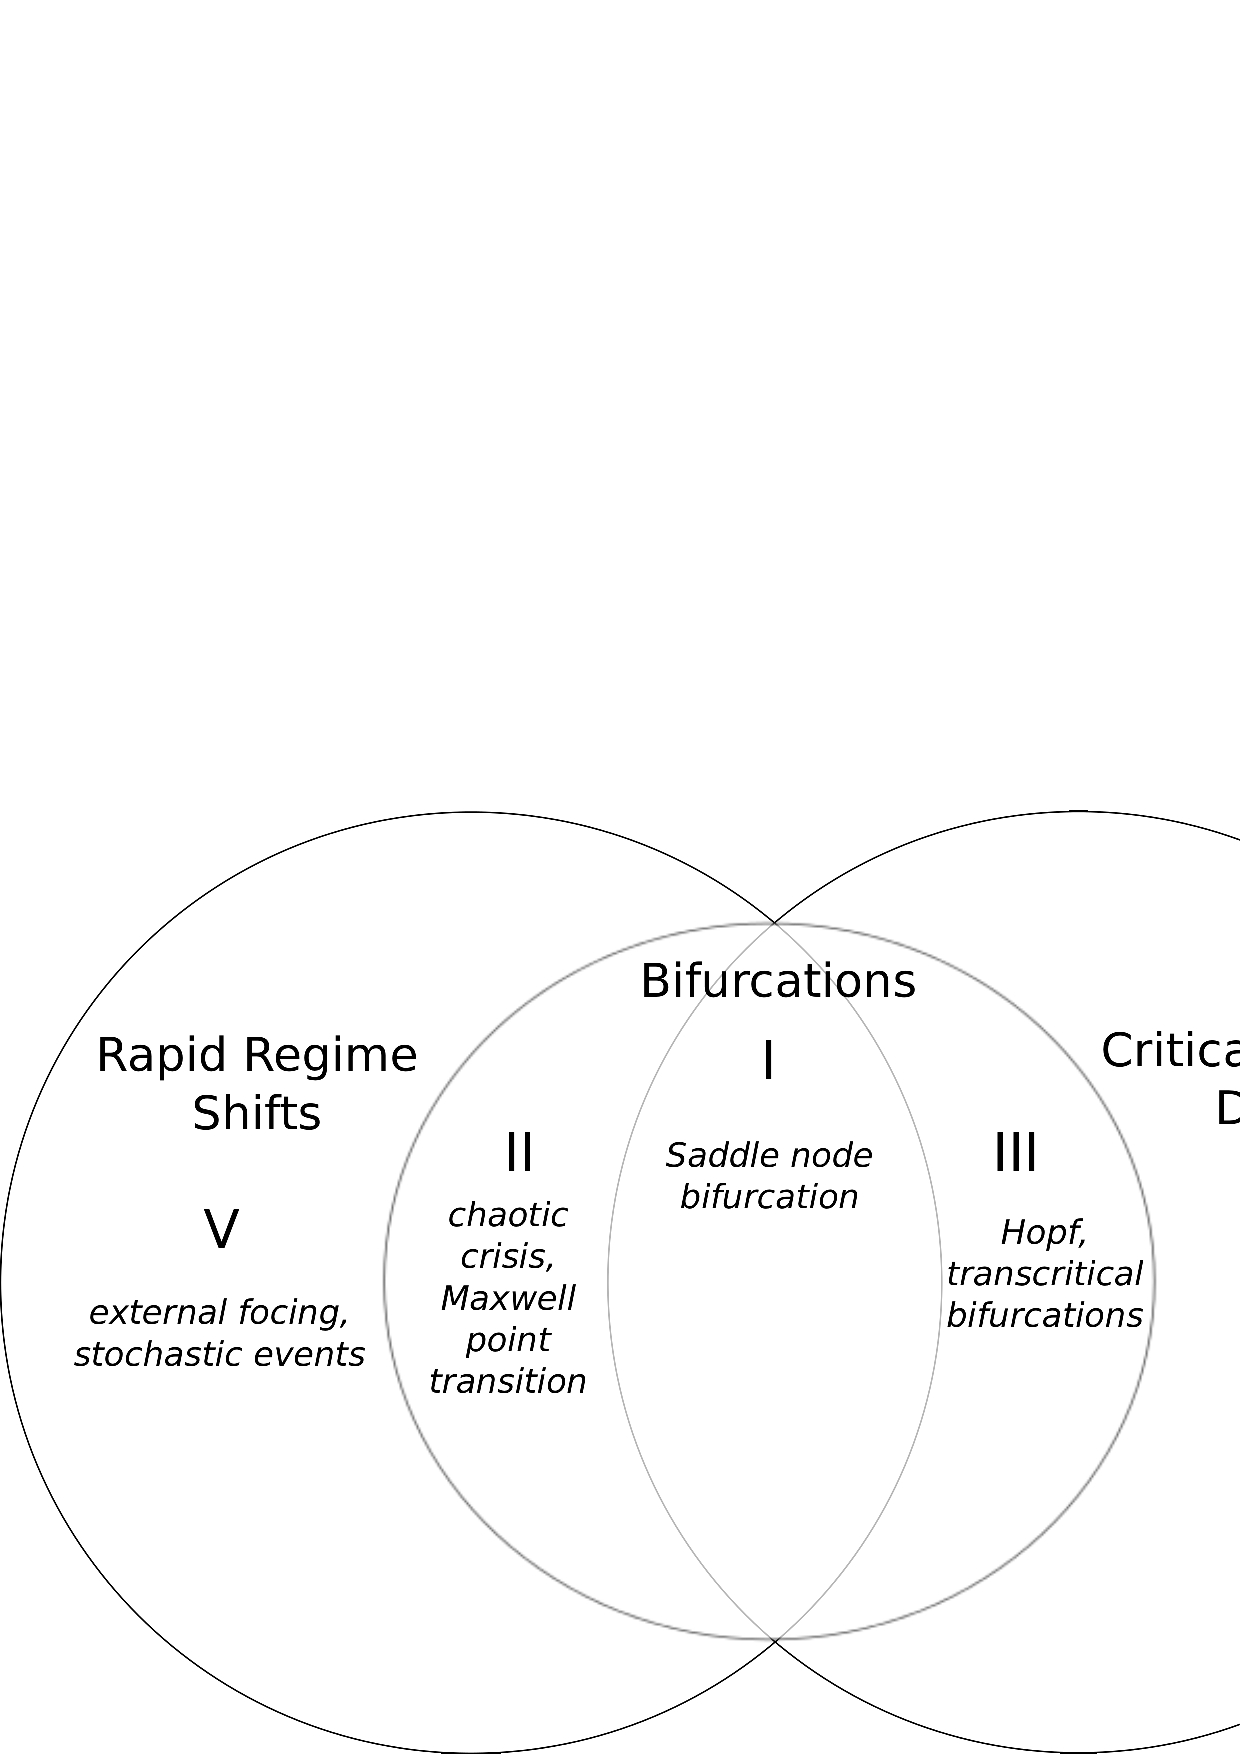
\includegraphics{ews-venn.pdf}
\caption{Venn diagram representing the intersecting domains of rapid
regime shifts, bifurcations, and critical slowing down. Labels in italic
are example phenomena that occur in each domain. Roman numerals indicate
example literature (right) exploring each domain, and also refer to
sections below describing those domains. The center domain, where all
three phenomena intersect, is the most extensively researched domain of
the EWS field.}
\end{figure}

\subsection{Catastrophic Bifurcations Preceded by CSD (I)}

Much of the (most visible) recent research in EWS has focused on the
center of the diagram, where all three concepts intersect. The warning
signal patterns postulated, such as increasing variance and coefficient
of variation, (Carpenter, Bennett, and Peterson 2006), increasing
autocorrelation (Dakos et al. 2008), increasing skewness (Guttal and
Jayaprakash 2008) can all be directly derived from the changing
eigenvalue in a saddle node bifurcation. Consequently, experimental
evaluations of warning signals have largely focused on this situation as
well. CSD has frequently been studied in the context of models
exhibiting a saddle-node bifurcation.

Dai et al. (2012) maps out the entire saddle-node bifurcation diagram
empirically before presenting the corresponding decrease in recovery
time (increase in variance and autocorrelation over time). Veraart et
al. (2011) shows a very similar result in a similar system. These
important experiments are among the best demonstrations that saddle-node
bifurcation dynamics really occur in natural systems, and can be
accompanied by reliable detection of EWS, at least when sufficient data
sampling, replicates, and controls are available.

Carpenter et al. (2011) provides an even more ambitious example, in
which a lake ecosystem is manipulated towards a sudden transition
through the introduction of a predator, while a neighboring experimental
lake provides a control. In this example, the underlying dynamics of a
whole lake ecosystem are far less tractable than the laboratory
controlled chemoststats of microorganisms. While it is more difficult to
identify the bifurcation process, the system is understood well enough
to anticipate that a sudden transition can be induced under the intended
manipulation. Like the laboratory examples, this helps eliminate the
options outside the circle ``bifurcations,'' in Figure 1. The observed
warning signals then place it in the center of the diagram.

While these studies have provided valuable demonstrations of the
potential to find early warning signals of sudden transitions, this
literature has begun to enumerate examples of similar transitions in
which no such signal is present.

\subsection{Catastrophic Bifurcations \emph{not} Preceded by CSD (II)}

Saddle nodes are only one of a variety of bifurcations, which can cause
rapid changes in system dynamics. Other bifurcations can cause long-term
changes in system dynamics without a gradual pass through a state with
zero eigenvalue, and therefore, not exhibit CSD. Many of these examples
can in fact show patterns in typical early warning indicator variables
such as variance or autocorrelation that are completely opposite to the
patterns seen in the saddle-node case.

These are some of the most problematic cases. They represent disruptive
but potentially avoidable events, but would not be detected by using CSD
as an EWS. These cases include bifurcations in continuous time
{[}@Schrieber2008{]} and discrete time {[}@Schrieber2003{]}, explicitly
spatial (Bel, Hagberg, and Meron 2012) and non-spatial, chaotic
(Schreiber 2003, ) and non-chaotic (Hastings and Wysham 2010, , )
examples. Before warning signals can be reliably applied to novel
systems, research must provide a way to discern if the dynamics
correspond to the more well understood warning signals of the
saddle-node case or the more complex patterns such as the examples
discussed here.

One class of bifurcations in which we would not expect to see CSD prior
to regime shift are sometimes known as \emph{crises}. Crises are sudden
changes in the dynamics of chaotic attractors that occur in response to
small changes in parameters (Grebogi, Ott, and Yorke 1983). Chaotic
attractors are features of many ecological models (Hastings et al.
1993), and chaotic behavior has been shown in some ecological systems
{[}@Constantino1997{]}.

Hastings and Wysham (2010) examined a continuous model of a stochastic
three-species food chain where all species migrate between six patches.
When environmental stochasticity (represented as random variation in the
carrying capacity) is low, all species coexist in a chaotic but stable
attractor. A small increase in environmental stochasticity, though,
causes extinction of the top predator and rapid shift to a non-chaotic
cycle. Despite an increase in environmental variability, neither the
variance nor skew of the populations of any species change as the system
approaches this bifurcation.

Another example of a chaotic crisis can be found in a simple
discrete-time model where a population is subject to strong density
dependence (an Allee effect) and harvested by predators with a Type II
(saturating) functional response (Schreiber 2003). When prey have high
growth rates, the system has chaotic dynamics. Small increases in the
predation intensity cause a bifurcation with chaotic but persistent prey
populations to prey extinction. As predation intensity increases towards
this threshold, the population exhibits \emph{decreasing} variance.

\begin{figure}[htbp]
\centering
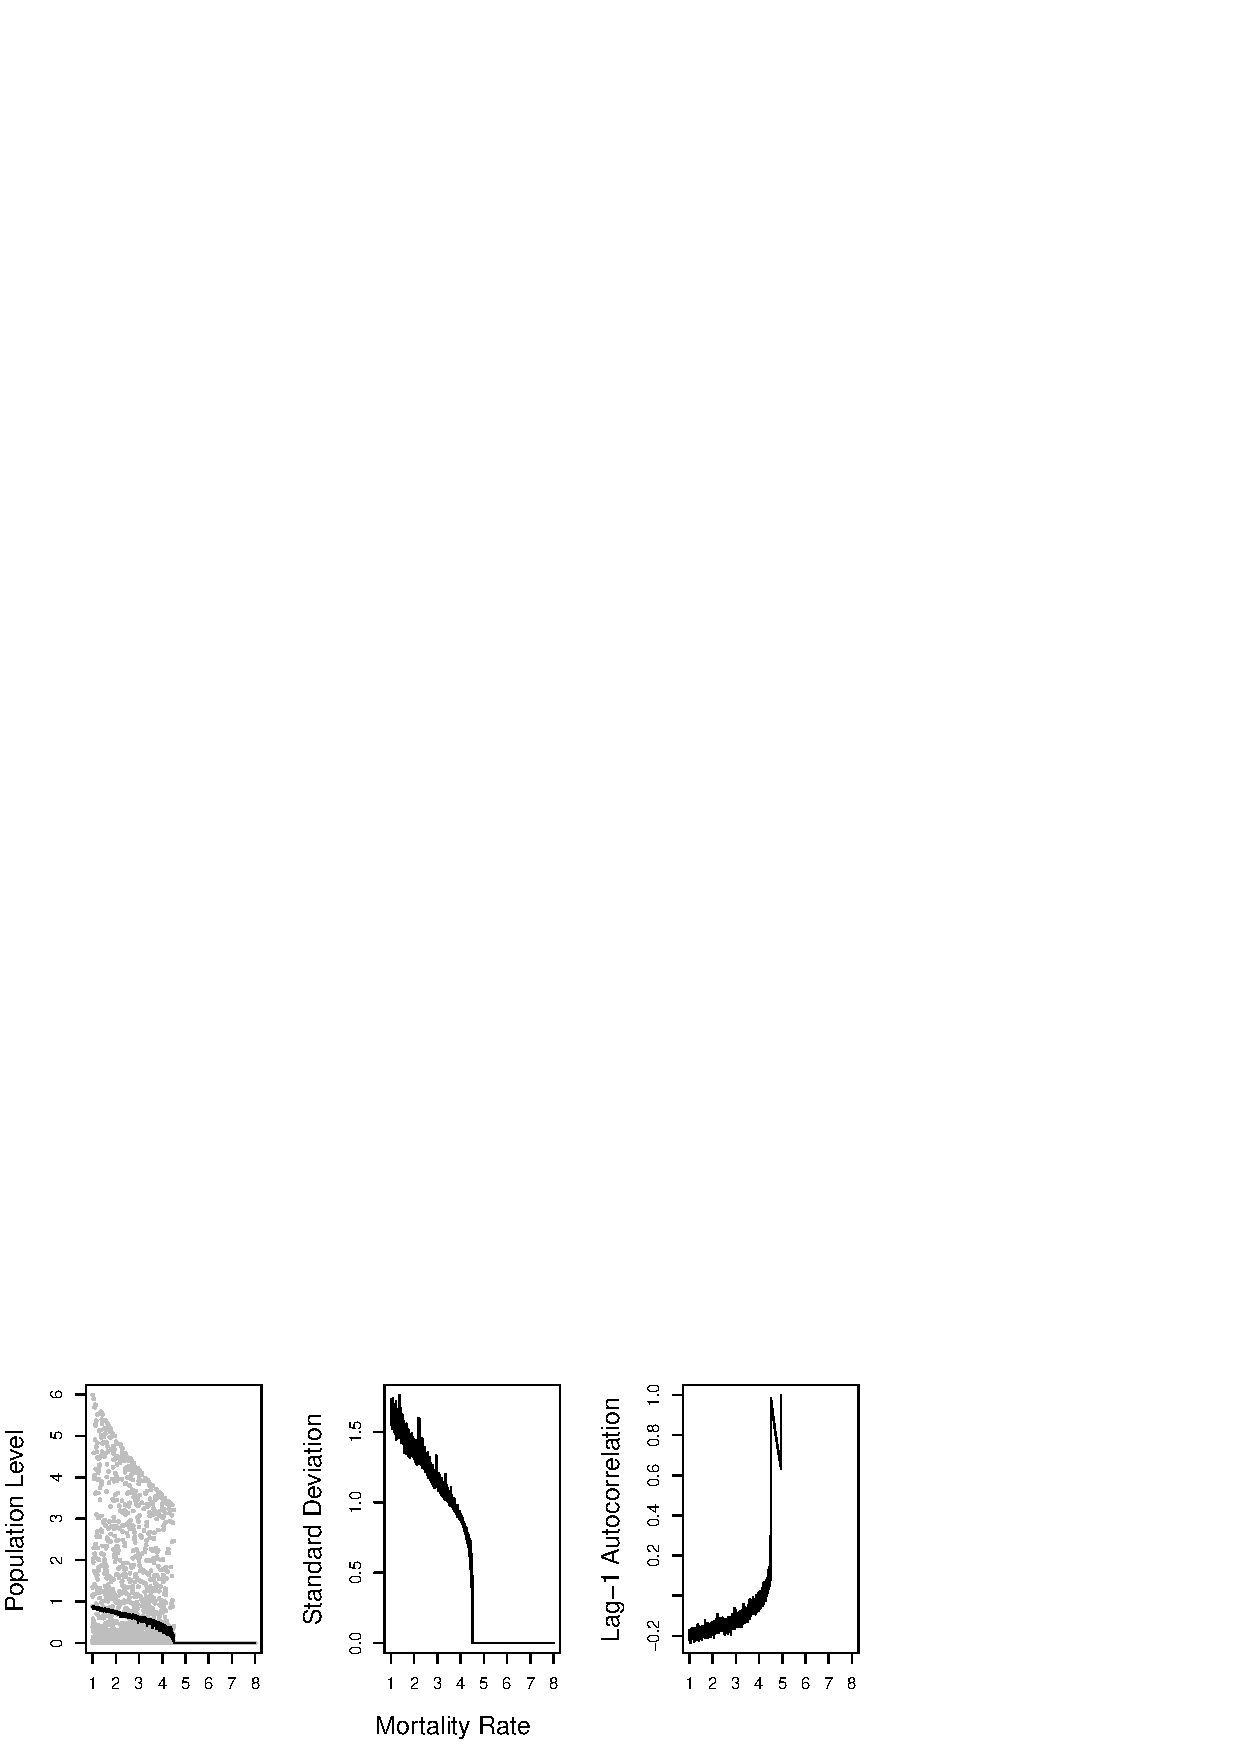
\includegraphics{schreiber-fig.pdf}
\caption{A system where variance decreases prior to a population
collapse; adapted from Schreiber (2003). In this model, prey species
with high growth rates exhibit chaotic dynamics under predation, but
populations collapse when predation increases beyond a threshold value.
Left: The population level as a function of predation rate. Middle:
Variance of the prey population level. Note that it \emph{decreases} as
predation rate approaches the threshold. Right: Lag-1 Autocorrelation in
prey population dynamics increases as the threshold is approached}
\end{figure}

Examples are not restricted to chaotic dynamics. Some spatially extended
systems exhibit a type of bifurcation that is not accompanied by CSD. In
one class of models, individual locations are subject to saddle
node-type regime shifts and influence adjacent locations via short-range
facilitation and long-range competition. Such models are used represent
transitions between vegetation types in response to changing water
availability, and reproduce naturally occurring vegetation patterns
(Rietkerk and van de Koppel 2008). In such systems, a regime shift in
one location can propagate spatially and transition the whole system
from one regime to another. Such a transition occurs if the control
parameter (e.g., rainfall), exceeds the \emph{Maxwell point} - the value
at which a local disturbance propagates outwards (Bel, Hagberg, and
Meron 2012). The Maxwell point may be far from the level at which an
individual location would undergo a saddle-node bifurcation, and thus
the system's global dynamics would not exhibit CSD prior to such a
transition. Another example is found in Schreiber and Rudolf (2008)., in
which variance is observed to decrease before a sudden transition that
follow a Hopf bifurcation .

\subsection{Non-Catastrophic Bifurcations Preceded by CSD (III)}

Not all regime shifts are rapid. Some systems undergo bifurcations
between qualitatively different, but quantitatively similar regimes.
These transitions may be reversible. In a management setting, such
qualitative changes may insignificant, so warning signals that detect
such transitions may be effective ``false positives.''

CSD precedes several types of these non-catastrophic bifurcations. In
the subcritical form of a Hopf bifurcation, a system transitions from a
stable equilibrium to a stable cycle. This bifurcation occurs in
classical predator-prey systems (May 1972) and has been observed in
experimental systems (Drake and Griffen 2010; J. Carpenter 2011; Veraart
et al. 2011; Dai et al. 2012; Wang et al. 2012). As a control parameter
approaches the critical threshold, the system's dominant eigenvalue
approaches zero and thus exhibits CSD (Chisholm and Filotas 2009; Kéfi
et al. 2012). However, the mean value of the equilibrium does not change
dramatically, and the transition from stable equilibrium to cycles is
gradual as the cycle sizes grow from zero at the threshold value. In the
presence of stochasticity, system behavior may be observed on either
side of the threshold may be indistinguishable.

The system's eigenvalue also passes through zero in the case of the
transcritical bifurcation. The transcritical is a degenerate case of the
saddle-node, and occurs in many of the same systems. However, when a
system passes through a transcritical bifurcation, the stable
equilibrium transitions smoothly from positive to zero, or the reverse.
In population systems, this corresponds to a transition from an
equilibrium of a very small population size to extinction - an important
but non-catastrophic, and probably directly observable, event. CSD is
observed prior to the transcritical bifurcations (Chisholm and Filotas
2009; Kéfi et al. 2012).

An experimental example a transcritical bifurcation found in Drake and
Griffen (2010), where a population of \emph{Daphnia} was forced through
a transcritical bifurcation by reducing food supplies and driving
population growth rates below zero. Indicators of CSD (variation,
skewness, autocorrelation, and spatial correlation) increased prior to
collapse of the population.

\subsection{CSD in the absence of bifurcations or regime shifts. (IV)}

Critical slowing down may appear in systems without any bifurcations.
Kéfi et al. (2012) showed that smooth transitions that modify a system's
potential and decrease the value of its dominant eigenvalue would result
in longer return times and greater variance and autocorrelation in
system behavior (See Figure 3). When the transition between states is
smooth, these measures will exhibit a smooth increase to a maximum and
then a decrease, unlike the sharp peaks found in systems with
bifurcations. Nonetheless, both exhibit increasing measures of CSD that
may be indistinguishable.

\begin{figure}[htbp]
\centering
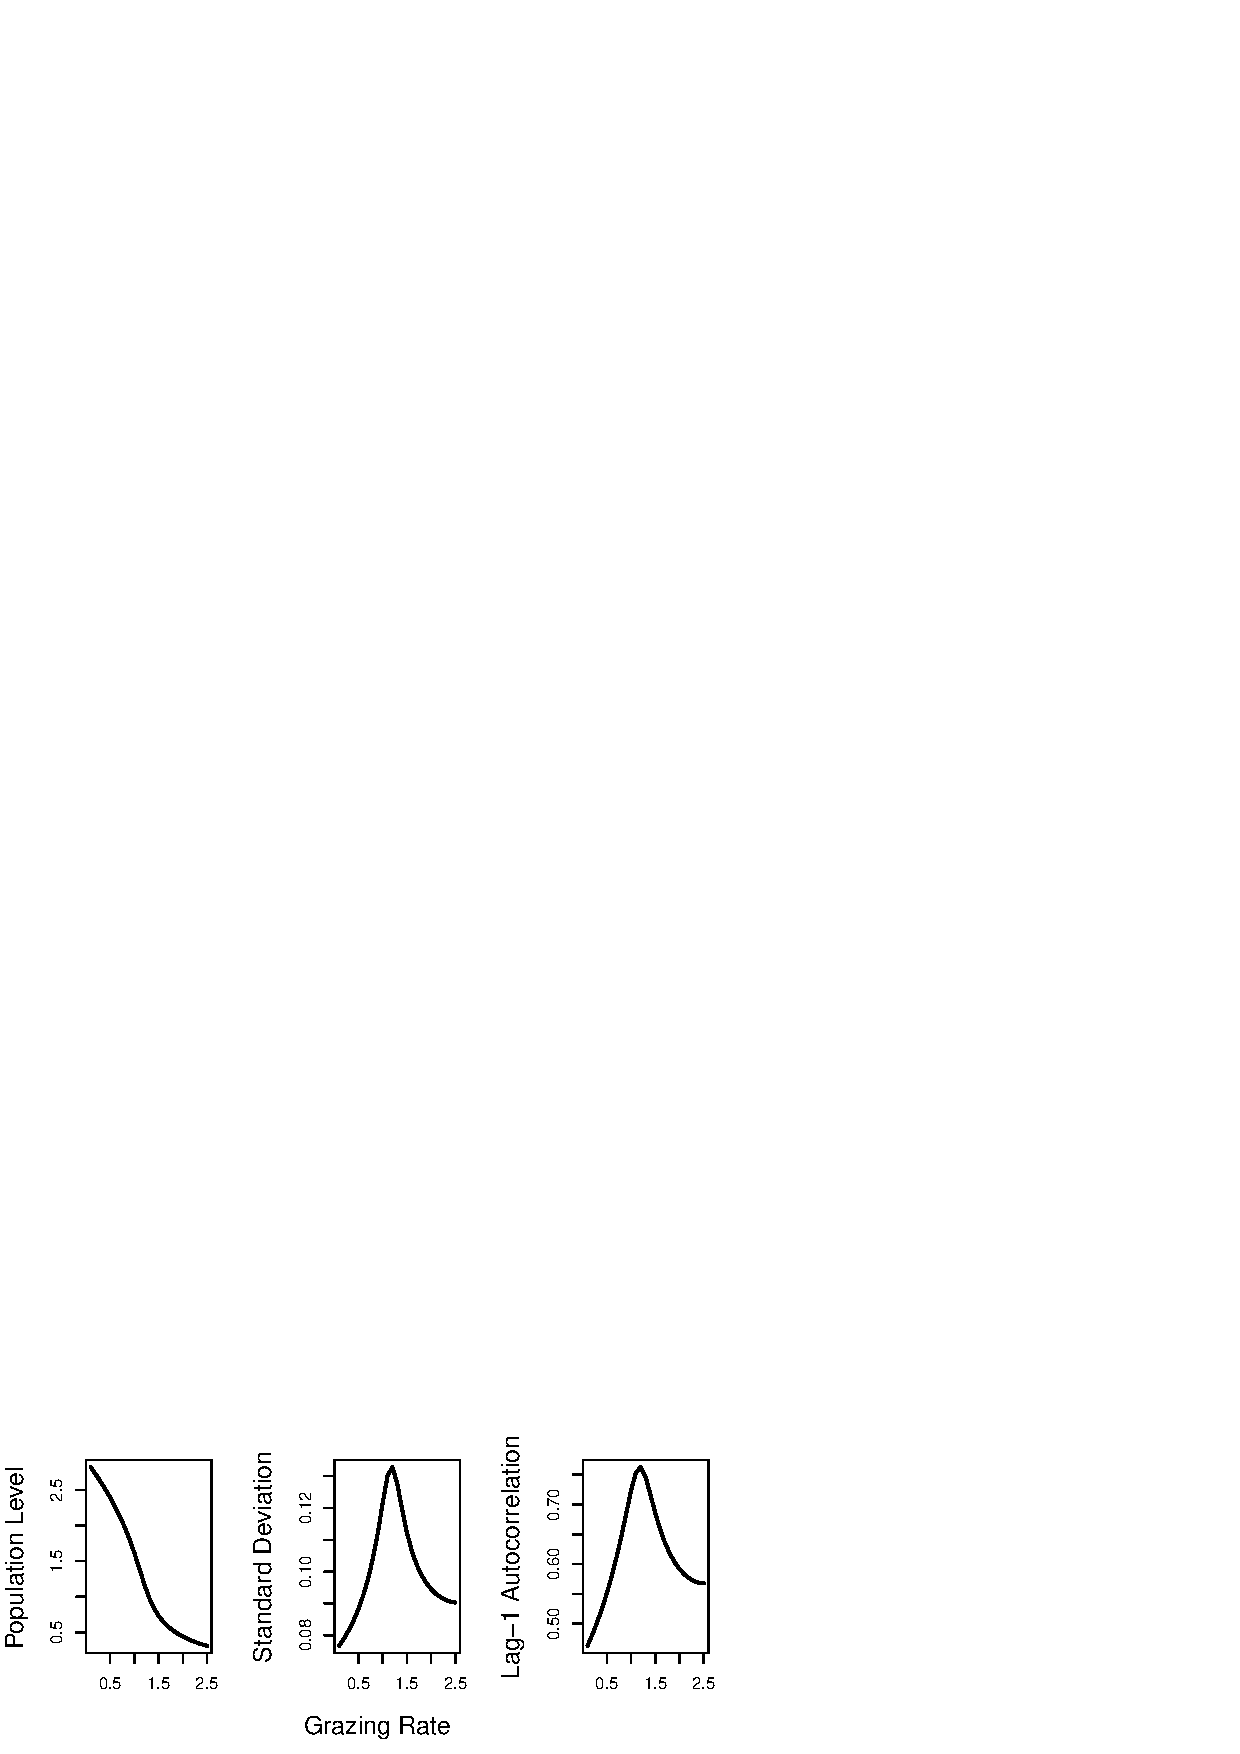
\includegraphics{kefi-fig.pdf}
\caption{A system where critical slowing down is observed without a
critical threshold, from Kéfi et al. (2012). In this model, prey have
logistic growth and are subject to predation with a Type III functional
response, but there is no bifurcation. Instead, average prey population
exhibits a smooth response to increased predation. Left: The population
level as a function of predation rate. Middle: Variance of the prey
population level. Note that it increases during the transition, despite
no bifurcation. Right: Lag-1 Autocorrelation in prey population dynamics
as predation rate increases. Note that it, too, increases despite the
lack of a bifurcation}
\end{figure}

\subsection{Non-Catastrophic Bifurcations without CSD (V)}

Some bifurcations involve neither catastrophic shifts nor patterns of
critical slowing down. The transition from very small populations to
zero is one such transition. System behavior after extinction is clearly
different, and exhibits hysteresis. However, the transition, while not
smooth, is not due to a saddle-node or similar bifurcation, and CSD
would not be expected.

\subsection{Catastrophic Regime Shifts without Bifurcations or CSD (VI)}

Some rapid regime shifts are not due to bifurcations at all. A large
external forcing (as illustrated in Figure 4) may change the behavior of
a system without any warning. This mechanism is commonly recognized,
(Barnosky et al. 2012; Scheffer et al. 2001; Scheffer et al. 2009;
Scheffer et al. 2012), but others are possible. An internal stochastic
event may switch a system between dynamic regimes, or a change in system
behavior may be the manifestation of a long-term transient. In none of
these cases would CSD be expected to precede such changes.

\begin{figure}[htbp]
\centering
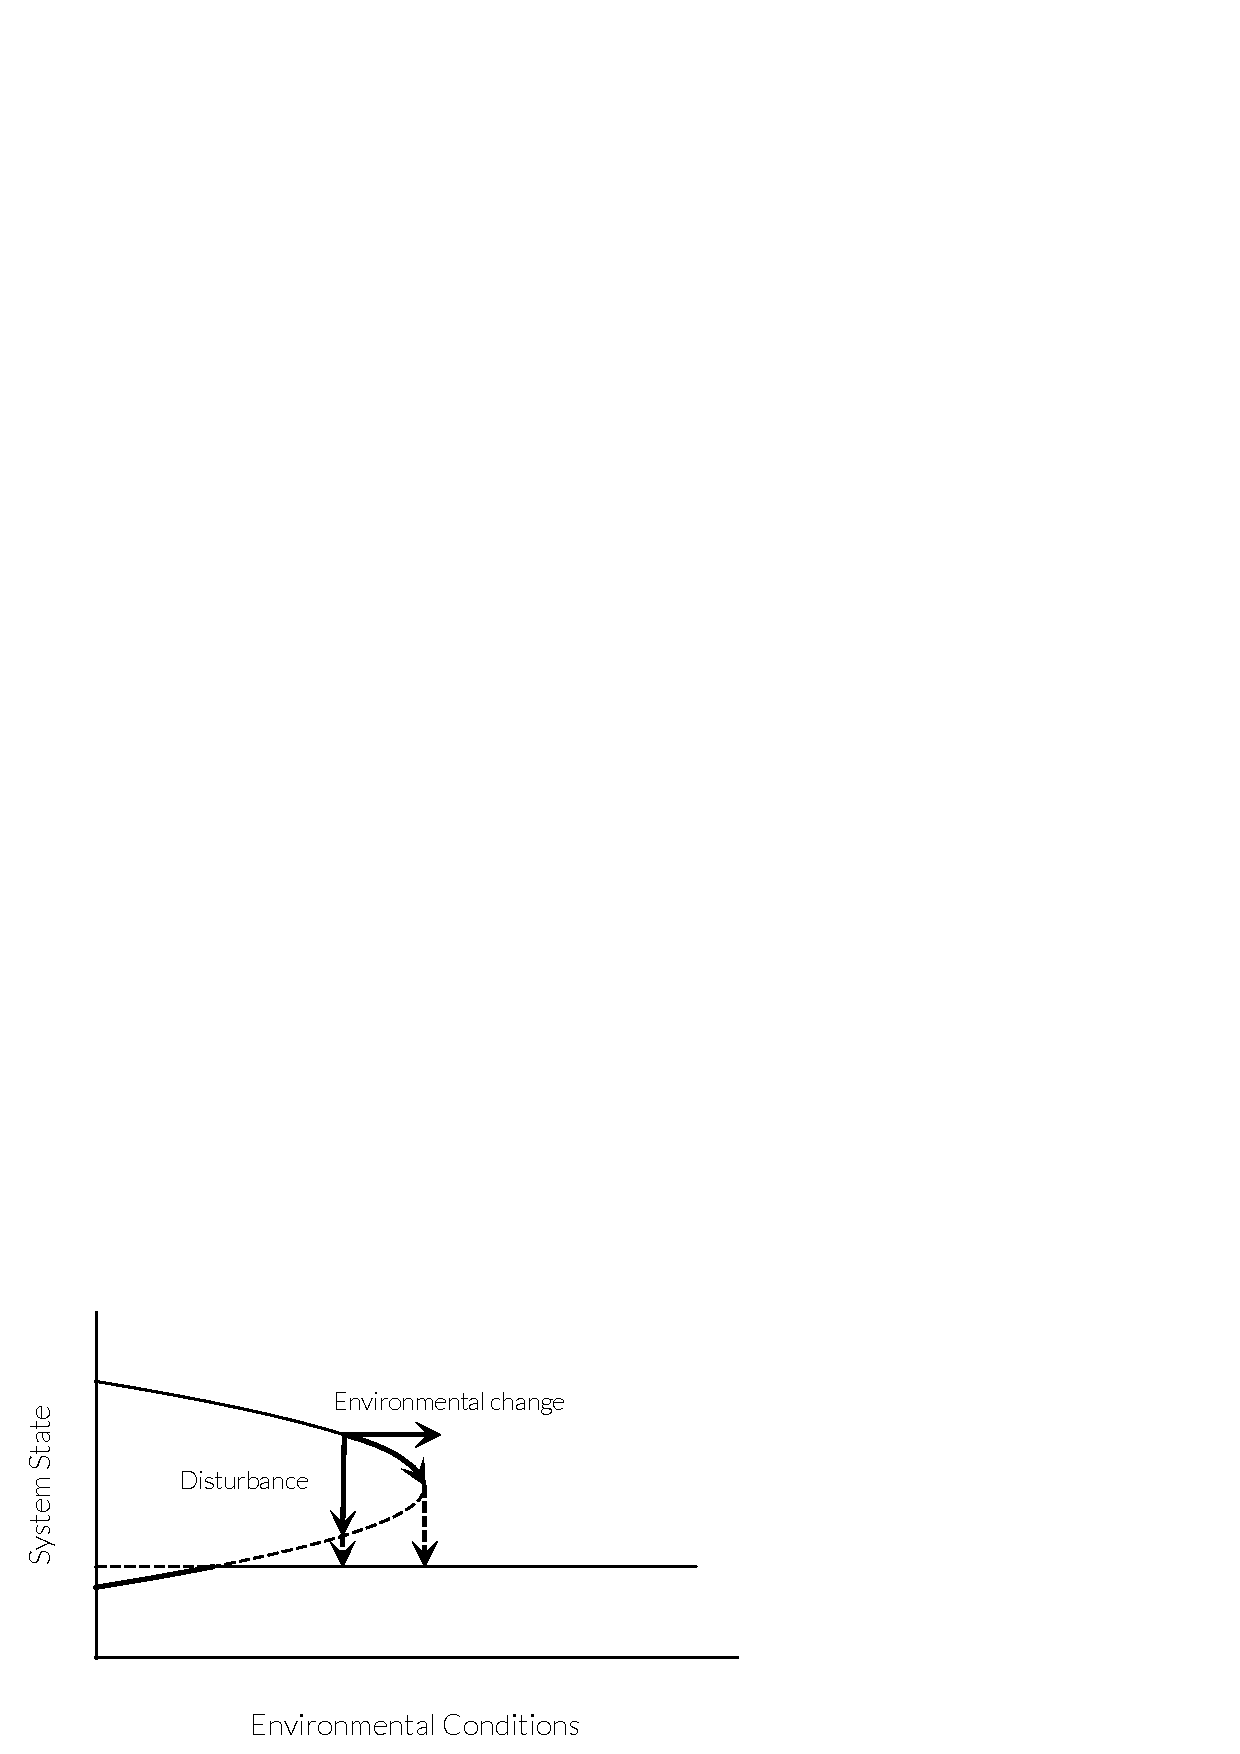
\includegraphics{Bel2012example.pdf}
\caption{Difference between different types of perturbations. On the
horizontal axis is the bifurcation parameter, representing the state of
the environment (e.g.~annual mean temperature) whose slow change could
lead to a sudden shift. A direct disturbance to the system state
(e.g.~population size, vertical axis) could also cause a transition if
it is large enough to cross the stability threshold (dashed line). Such
a perturbation can come from exogenous factors such as anthropogenic
pressures or occur by chance from intrinsic stochasticity. These
distinct mechanisms of disturbance and environmental change are coupled
-- as the environment deteriorates, moving the system right on the
diagram, the probability that a disturbance crosses the threshold
increases. From Bel, Hagberg, and Meron (2012).}
\end{figure}

Large, rapid changes in external conditions will result in rapid changes
in ecological system dynamics. For instance, rapid changes in North
American vegetation at the start of the Bølling-Allerød and end of the
Younger Dryas period are thought to be responses to similarly large,
rapid changes in climate (Williams, Blois, and Shuman 2011). Doney and
Sailley (2013) interpret a recent analysis by Di Lorenzo and Ohman
(2013) as demonstrating that what were previously thought of as regime
shifts in krill dynamics in the Pacific ocean (Hare and Mantua 2000)
could actually be explained by a close coupling to El Nino environmental
dynamics through the Pacific Decadal Oscillation (PDO).

Stochastic perturbations may shift systems from one regime to another
even if underlying environmental conditions remain the same. Hastings
and Wysham (2010) showed that in a model where one species with
stochastic Ricker dynamics disperses among eight patches, model behavior
can switch stochastically between wildly oscillatory behavior and
regularly cycling regimes even while parameters (including stochastic
variability) remain the same.

Schooler et al. (2011) found that lakes with the invasive plant
\emph{Salvaniai molesta} and herbivorous weevils alternated between low-
and high-\emph{Salvnia} states driven by external disturbances from
regular flooding events. Ditlevsen and Johnsen (2010) examined 25 abrupt
climate changes that occurred during the last glacial period
(Dansgaard-Oeschger events) and found no evidence for CSD in
high-resolution climate data from ice cores, and concluded that the
events were driven by endogenous climate stochasticity.

Some events that appear to be regime shifts may actually be transients
in some systems. Sudden changes in dynamics can occur in simple
ecological models with strong density dependence that take long times to
reach equilibrium. Hastings (1998) showed such dynamics in model of
dispersal of inter- or sub-tidal organisms whose larvae disperse along a
coastline. Over the thousands of years it takes the model to reach
equilibrium, it may alternate between temporary regimes of regular
cycles and chaos that switch in only a few years. While on long time
scales these are technically not regime shifts, such changes would
effectively appear to be regime shifts on shorter ones. We would not
expect such regime shifts to be preceded with CSD.

\section{Statistical problems in detecting early warning signals}

The above cases show that behavior providing an early warning signal
before regime shifts may only be present in certain types of ecological
systems. An additional important consideration is whether these
behaviors will be \emph{detectable} in those domains where they are
expected. To be usable as an EWS, system behavior must be detectable
well enough in advance of a regime shift to serve in decision-making,
and be reliably distinguishable from other patterns.

Ecological data is often sparse, noisy, autocorrelated and subject to
confounding driving variables, in contrast to much of the experimental
or simulated data used to test EWS. Under common levels of noise found
in field data, CSD-based EWS often fail (Perretti and Munch 2012).

A wide variety of statistical summary indicators have been examined as
potential detectors of CSD. The most common are variance and
autocorrelation. Others include skewness {[}Guttal2008a{]} and
conditional heteroscedasticity (Seekell, Carpenter, and Pace 2011).
These statistics are typically calculated on sliding windows of
time-series data and tested formally or informally for trends. The
relative power of these tests varies considerably with context; no
indicator has consistently outperformed others (Perretti and Munch 2012;
Lindegren et al. 2012; V. Dakos, van Nes, et al. 2011; Dakos et al.
2012). Also, measuring these indicators requires making sometimes
arbitrary calculations. For instance, the power of lag-1 autocorrelation
to detect a regime shift may be modified by changing methods of data
aggregation, de-trending, changing sliding window length, filtering
signal bandwidth (Lenton et al. 2012). These choices may be optimized
when enough calibration data is available, as Lenton et al. (2012) were
able to do with several sets of paleoclimate data. However, such
calibration may not be possible with many ecological datasets.
Multiple-method (Lindegren et al. 2012) and composite indices (Drake and
Griffen 2010) have been proposed, but their power relative to other
indicators is unknown.

Another approach to detecting CSD has been fitting time series data to
models. Two approaches have been used for these model-based methods.
First, models may be used to calculate summary statistics related to
CSD, such as eigenvalues (Lade and Gross 2012) or diffusion terms in
jump-diffusion models (Stephen R. Carpenter 2011; Brock and Carpenter
2012). These statistics are then examined for trends in the same fashion
as the summary statistics above. Alternatively, models representing both
deteriorating and stable conditions may be fit to the data and in order
to determine which is more likely (Dakos et al. 2012, ). Carl Boettiger
and Hastings (2012) found that likelihood ratio tests were more powerful
than trend-based summary statistic tests across several real and
simulated ecological data sets. This approach is also more robust than
summary-statistic methods to spurious correlations that arise when
collapses are driven by purely stochastic events (C. Boettiger and
Hastings 2012)

Care is required in the criteria used to judge the power of warning
signal methods. The trade-off between false negatives and false
positives is a matter of not just statistical but economic efficiency.
For instance, a large number of false positives may be acceptable if
they reduce the probability of a false warning that would result in an
otherwise avoidable catastrophic regime shift, and the costs of failing
to detect such a shift exceed that of the false positives. Carl
Boettiger and Hastings (2012) suggest the use of receiver-operating
characteristic (ROC) curves to describe the performance of various EWS.
ROC curves (Figure 5) represent the false positive rate at any true
positive rate. The area under the curve (AUC) is a useful metric of
overall performance. AUC will be one if the signal is perfect and 0.5 if
the signal performs no better than random. The complete shape of the
curve provides more information on the possible trade-offs under
different sensitivities. This information, combined with a
decision-theoretic framework, has the potential to illuminate in which
cases EWS can be useful.

\begin{figure}[htbp]
\centering
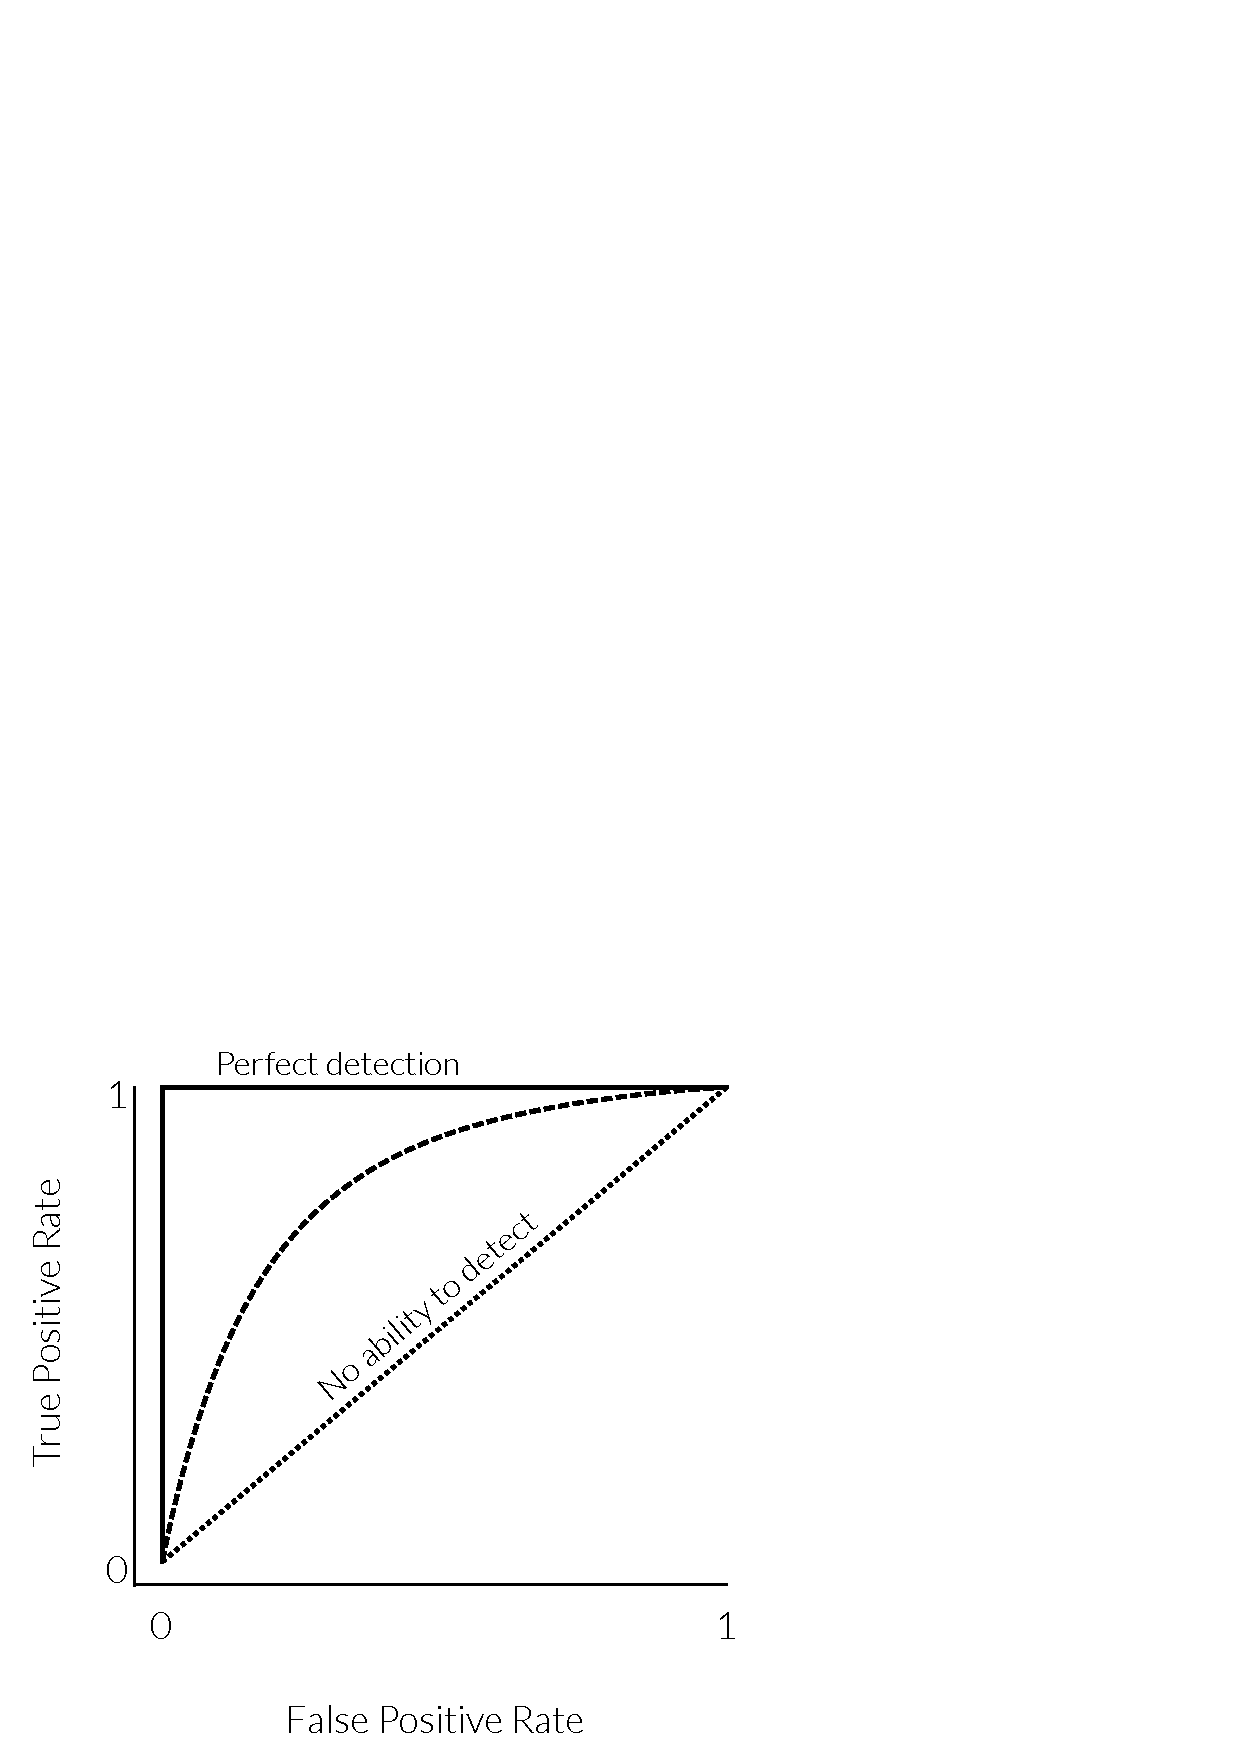
\includegraphics{ROC.pdf}
\caption{Receiver-operating characteristic (ROC) curves illustrate the
trade-off between false positive and true positive detection rates of an
EWS. Perfect warning signals (solid curve) would identify all thresholds
while generating no false positives, while very poor signals would have
no ability to distinguish false from true signals (dotted line). In
reality, warning signals' have a trade-off between the two which is
described by a curve (dotted line) or summarized by the area under the
ROC curve}
\end{figure}

\section{Discussion}

Recognizing the potential for early warning signals of critical
transitions represents a substantial leap forward in addressing one of
the most challenging questions in ecology and ecosystem management
today. In the decades prior, the prospect that ecosystems could make
sudden transitions into an undesirable state due to gradual, slow
changes in their environment hung like a specter over both our
understanding and management of natural systems. Research that points to
the possibility of detecting these transitions holds the promise of
meeting this challenge and has attracted justifiably widespread
attention among both theoretical and empirical communities. Nonetheless,
our understanding of early warning signals is still in its infancy. Thus
far, our best understanding and empirical experience lies in transitions
that are driven by saddle-node (also called fold) bifurcations.

While saddle-node bifurcations may be common, they represent only part
of the potential mechanisms for rapid regime shift. Occupying the center
of our diagram, Figure 1, such transitions represent our best-understood
cases. Researchers have relied on existing expertise and prior research
to identify empirical systems most likely to experience critical
transitions through the saddle-node-like mechanism (e.g. J. Carpenter
2011; Dai et al. 2012), and have achieved a close match to theoretical
predictions of early warning signals. While these examples provide a
much needed proof-of-principle that these signals can be detected in the
real world, it is too early to apply the same methods to novel systems
where the saddle-node is only one of many possible mechanisms.

Thus, establishing the saddle node mechanism a necessary condition of
using CSD as a warning signal. This can be done via manipulation in
simple experimental systems (Veraart et al. 2011; Dai et al. 2012), but
this is impractical in nature. Another approach is to assume the
saddle-node mechanism applies to a limited set of systems that have
well-studied examples, such as lakes undergoing eutrophication (Scheffer
et al. 2001), or forest/savannah transitions may also (Staver,
Archibald, and Levin 2011; Hirota et al. 2011; Bel, Hagberg, and Meron
2012). Fitting simplified saddle-node models, following Carl Boettiger
and Hastings (2012) to past regime shifts in less well-understood
systems may provide evidence for the mechanism. However, care must be
taken to specify sufficient alternative models.

CSD alone cannot be used as evidence regime shift. In some cases, it
will be present when no transition is approaching. In other cases,
regime shifts occur without CSD. Though false alarms and missed events
can occur in any statistical procedure, the cases discussed here
demonstrate that these errors will also arise when the underlying
dynamics do not correspond to our assumptions. These situations fall in
the uncharted area beyond the center of Figure 1, where research has
just begun to illuminate their existence. A better theoretical and
empirical understanding of these cases will allow us to construct novel
warning signals, that may be opposite the patterns observed in the
familiar saddle-node bifurcations. Before early warning signals can be
applied in novel systems, additional information is needed in order to
determine best signal to use.

The future of early warning signals lies in the uncharted territory. For
certain classes of transitions, such as stochastically-driven regime
shifts, prediction may not be possible. In such cases, managing for
resilience may be the only option. Likewise, regime shifts driven by
external perturbation or strong forcing are not predictable \emph{if}
the scope of management does not include the external causes. Proper
scoping of the management problem can avoid this situation (Alliance
2010; Fischer et al. 2009; Polasky et al. 2011).

For other classes of transitions, prediction may be possible but other
EWS must be explored. Flickering (Brock and Carpenter 2010; Wang et al.
2012), or rapid transitions between states prior to a more permanent
transition, is one signal that may apply across many types of systems.
It manifests in bi-modality and high variance in times series. Spatial
pattern development may be a warning signal in systems with
short-distance positive feedbacks but long-distance negative feedbacks,
such as grassland-desert transitions (van Nes and Scheffer 2005; Kéfi et
al. 2007, ). Other spatial signals may apply where systems include both
saddle nodes and positive feedbacks across space (Guttal and Jayaprakash
2008; Litzow, Urban, and Laurel 2008; Dakos et al. 2009; Bailey 2010; V.
Dakos, van Nes, et al. 2011; Bel, Hagberg, and Meron 2012). A critical
task for EWS research is to map these signals to their domains of
applicability, and create methods to establish if ecosystems fall into
these domains.

\section{Acknowledgments}

This work was partially supported by the Center for Stock Assessment
Research, a partnership between the University of California Santa Cruz
and the Fisheries Ecology Division, Southwest Fisheries Science Center,
Santa Cruz, CA, to CB; the NSF Integrative Graduate Education and
Research Traineeship Program to NR and by funding from NSF Grant EF
0742674 to AH.

\section{References}

Alliance, Resilience. 2010. \emph{Assessing Resilience in
Social-Ecological Systems : Workbook for Practitioners. Version 2.0}.
\url{http://www.resalliance.org/3871.php}.

Bailey, R. M. 2010. ``Spatial and temporal signatures of fragility and
threshold proximity in modelled semi-arid vegetation.''
\emph{Proceedings. Biological sciences / The Royal Society} (October)
(oct). doi:10.1098/rspb.2010.1750.
\url{http://www.ncbi.nlm.nih.gov/pubmed/20943693}.

Barnosky, Anthony D., Elizabeth a Hadly, Jordi Bascompte, Eric L.
Berlow, James H. Brown, Mikael Fortelius, Wayne M. Getz, et al. 2012.
``Approaching a state shift in Earth's biosphere.'' \emph{Nature} 486
(7401) (jun): 52--58. doi:10.1038/nature11018.
\url{http://dx.doi.org/10.1038/nature11018}.

Bel, Golan, Aric Hagberg, and Ehud Meron. 2012. ``Gradual regime shifts
in spatially extended ecosystems.'' \emph{Theoretical Ecology} 5 (4)
(jan): 591--604. doi:10.1007/s12080-011-0149-6.
\url{http://dx.doi.org/10.1007/s12080-011-0149-6}.

Boettiger, C., and A. Hastings. 2012. ``Early warning signals and the
prosecutor's fallacy.'' \emph{Proceedings of the Royal Society B:
Biological Sciences} 279 (1748) (oct): 4734--4739.
doi:10.1098/rspb.2012.2085.
\url{http://dx.doi.org/10.1098/rspb.2012.2085}.

Boettiger, Carl, and Alan Hastings. 2012. ``Quantifying limits to
detection of early warning for critical transitions.'' \emph{Journal of
the Royal Society, Interface / the Royal Society} 9 (75) (oct):
2527--39. doi:10.1098/rsif.2012.0125.
\href{http://dx.doi.org/10.1098/rsif.2012.0125 http://www.ncbi.nlm.nih.gov/pubmed/22593100}{http://dx.doi.org/10.1098/rsif.2012.0125
http://www.ncbi.nlm.nih.gov/pubmed/22593100}.

Brock, William A., and Stephen R. Carpenter. 2010. ``Interacting Regime
Shifts in Ecosystems: Implication for Early Warnings.'' \emph{Ecological
Monographs} 80 (3) (aug): 353--367. doi:10.1890/09-1824.1.
\href{http://www.esajournals.org/doi/abs/10.1890/09-1824.1 http://www.esajournals.org/doi/abs/10.1890/09-1824}{http://www.esajournals.org/doi/abs/10.1890/09-1824.1
http://www.esajournals.org/doi/abs/10.1890/09-1824}.

Brock, William a, and Stephen R. Carpenter. 2012. ``Early Warnings of
Regime Shift When the Ecosystem Structure Is Unknown.'' Ed. Ricard V.
Solé. \emph{PLoS ONE} 7 (9) (sep): 45586.
doi:10.1371/journal.pone.0045586.
\url{http://dx.plos.org/10.1371/journal.pone.0045586}.

Carpenter, J. 2011. ``May the Best Analyst Win.'' \emph{Science} 331
(6018) (feb): 698--699. doi:10.1126/science.331.6018.698.
\url{http://www.sciencemag.org/cgi/doi/10.1126/science.331.6018.698}.

Carpenter, S. R., and W. a Brock. 2010. ``Early warnings of regime
shifts in spatial dynamics using the discrete Fourier transform.''
\emph{Ecosphere} 1 (5) (nov): 10. doi:10.1890/ES10-00016.1.
\url{http://www.esajournals.org/doi/abs/10.1890/ES10-00016.1}.

Carpenter, Stephen R. 2011. ``Early warnings of unknown nonlinear
shifts : a nonparametric approach.'' \emph{Ecology} 92 (12): 2196--2201.
\url{http://www.esajournals.org/doi/pdf/10.1890/11-0716.1}.

Carpenter, Stephen R., Elena M. Bennett, and Garry D. Peterson. 2006.
``Scenarios for ecosystem services: An overview.'' \emph{Ecology and
Society}.
\url{http://apps.isiknowledge.com/full\textbackslash{}_record.do?product=WOS\textbackslash{}\&search\textbackslash{}_mode=AdvancedSearch\textbackslash{}\&qid=1\textbackslash{}\&SID=U1ADlMa62oB3pn11jce\textbackslash{}\&page=1\textbackslash{}\&doc=18}.

Carpenter, Stephen R., J. J. Cole, M. L. Pace, R. Batt, W. a Brock, T.
Cline, J. Coloso, et al. 2011. ``Early Warnings of Regime Shifts: A
Whole-Ecosystem Experiment.'' \emph{Science} 1079 (April) (apr).
doi:10.1126/science.1203672.
\url{http://www.sciencemag.org/cgi/doi/10.1126/science.1203672}.

Carpenter, Stephen R., D. Ludwig, and W. A. Brock. 1999. ``Management of
eutrophication for lakes subject to potentially irreversible change.''
\emph{Ecological Applications} 9 (3): 751--771.
\url{http://www.esajournals.org/doi/full/10.1890/1051-0761(1999)009\%5B0751:MOEFLS\%5D2.0.CO\%3B2}.

Chisholm, Ryan a, and Elise Filotas. 2009. ``Critical slowing down as an
indicator of transitions in two-species models.'' \emph{Journal of
theoretical biology} 257 (1) (mar): 142--9.
doi:10.1016/j.jtbi.2008.11.008.
\url{http://www.ncbi.nlm.nih.gov/pubmed/19084025}.

Dai, L., D. Vorselen, K. S. Korolev, and J. Gore. 2012. ``Generic
Indicators for Loss of Resilience Before a Tipping Point Leading to
Population Collapse.'' \emph{Science} 336 (6085) (may): 1175--1177.
doi:10.1126/science.1219805.
\url{http://www.sciencemag.org/cgi/doi/10.1126/science.1219805}.

Dakos, Vasilis, Stephen R. Carpenter, William a Brock, Aaron M. Ellison,
Vishwesha Guttal, Anthony R. Ives, Sonia Kéfi, et al. 2012. ``Methods
for Detecting Early Warnings of Critical Transitions in Time Series
Illustrated Using Simulated Ecological Data.'' Ed. Bülent Yener.
\emph{PLoS ONE} 7 (7) (jul): 41010. doi:10.1371/journal.pone.0041010.
\url{http://dx.plos.org/10.1371/journal.pone.0041010}.

Dakos, Vasilis, Sonia Kéfi, Max Rietkerk, Egbert H. van Nes, and Marten
Scheffer. 2011. ``Slowing down in spatially patterned ecosystems at the
brink of collapse.'' \emph{The American naturalist} 177 (6) (jun): 153.
doi:10.1086/659945. \url{http://www.ncbi.nlm.nih.gov/pubmed/21597246}.

Dakos, Vasilis, Egbert H. Nes, Raúl Donangelo, Hugo Fort, and Marten
Scheffer. 2009. ``Spatial correlation as leading indicator of
catastrophic shifts.'' \emph{Theoretical Ecology} (nov): 163--174.
doi:10.1007/s12080-009-0060-6.
\url{http://www.springerlink.com/index/10.1007/s12080-009-0060-6}.

Dakos, Vasilis, Egbert H. van Nes, Paolo D'Odorico, and Marten Scheffer.
2011. ``Robustness of variance and autocorrelation as indicators of
critical slowing down.'' \emph{Ecology} (oct). doi:10.1890/11-0889.1.
\url{http://www.esajournals.org/doi/abs/10.1890/11-0889.1}.

Dakos, Vasilis, Marten Scheffer, Egbert H. van Nes, Victor Brovkin,
Vladimir Petoukhov, and Hermann Held. 2008. ``Slowing down as an early
warning signal for abrupt climate change.'' \emph{Proceedings of the
National Academy of Sciences} 105 (38) (sep): 14308--12.
doi:10.1073/pnas.0802430105.
\url{http://www.ncbi.nlm.nih.gov/pubmed/18787119}.

Di Lorenzo, Emanuele, and Mark D. Ohman. 2013. ``A double-integration
hypothesis to explain ocean ecosystem response to climate forcing.''
\emph{Proceedings of the National Academy of Sciences of the United
States of America} (jan). doi:10.1073/pnas.1218022110.
\url{http://www.ncbi.nlm.nih.gov/pubmed/23341628}.

Ditlevsen, Peter D., and Sigfus J. Johnsen. 2010. ``Tipping points:
Early warning and wishful thinking.'' \emph{Geophysical Research
Letters} 37 (19) (oct): 2--5. doi:10.1029/2010GL044486.
\url{http://www.agu.org/pubs/crossref/2010/2010GL044486.shtml}.

Doney, Scott C., and Sevrine F. Sailley. 2013. ``When an ecological
regime shift is really just stochastic noise.'' \emph{Proceedings of the
National Academy of Sciences of the United States of America} 110 (7)
(feb): 2438--2439. doi:10.1073/pnas.1222736110.
\url{http://dx.doi.org/10.1073/pnas.1222736110}.

Drake, John M., and Blaine D. Griffen. 2010. ``Early warning signals of
extinction in deteriorating environments.'' \emph{Nature} 467 (sep):
456--7. doi:10.1038/nature09389.
\url{http://dx.doi.org/10.1038/nature09389}.

Fischer, Joern, Garry D. Peterson, Toby A. Gardner, Line J. Gordon, Ioan
Fazey, Thomas Elmqvist, Adam Felton, Carl Folke, and Stephen Dovers.
2009. ``Integrating resilience thinking and optimisation for
conservation.'' \emph{Trends in ecology \& evolution} 24 (10): 549--554.
doi:10.1016/j.tree.2009.03.020.
\url{http://www.ncbi.nlm.nih.gov/pubmed/19665820}.

Gandhi, A., S. Levin, and S. Orszag. 1998. ```Critical slowing down' in
time-to-extinction: an example of critical phenomena in ecology.''
\emph{Journal of theoretical biology} 192 (3) (jun): 363--76.
doi:10.1006/jtbi.1998.0660.
\url{http://dx.doi.org/10.1006/jtbi.1998.0660}.

Grebogi, C., E. Ott, and J. A. Yorke. 1983. ``Crises, sudden changes in
chaotic attractors, and transient chaos.'' \emph{Physica D: Nonlinear
Phenomena}.
\url{http://www.sciencedirect.com/science/article/pii/0167278983901264}.

Guttal, Vishwesha, and C. Jayaprakash. 2008. ``Spatial variance and
spatial skewness: leading indicators of regime shifts in spatial
ecological systems.'' \emph{Theoretical Ecology} 2 (1) (dec): 3--12.
doi:10.1007/s12080-008-0033-1.
\url{http://www.springerlink.com/index/10.1007/s12080-008-0033-1}.

Guttal, Vishwesha, and Ciriyam Jayaprakash. 2008. ``Changing skewness:
an early warning signal of regime shifts in ecosystems.'' \emph{Ecology
letters} 11 (5) (may): 450--60. doi:10.1111/j.1461-0248.2008.01160.x.
\url{http://www.ncbi.nlm.nih.gov/pubmed/18279354}.

Hare, S. R., and N. J. Mantua. 2000. ``Empirical evidence for North
Pacific regime shifts in 1977 and 1989.'' \emph{Progress in
oceanography} 47 (2000): 103--145.
\url{http://www.sciencedirect.com/science/article/pii/S0079661100000331}.

Hastings, Alan. 1998. ``Transients in spatial ecological models.'' Ed.
Jordi Bascompte and Ricard V. Solé. \emph{Modeling spatiotemporal
dynamics in ecology}: 189--198.
\url{http://scholar.google.com/scholar?hl=en\textbackslash{}\&btnG=Search\textbackslash{}\&q=intitle:Transients+in+spatial+ecological+models\textbackslash{}\#0}.

Hastings, Alan, C. L. Hom, Stephen Ellner, Peter Turchin, and H. C. J.
Godfray. 1993. ``Chaos in ecology: is mother nature a strange
attractor?'' \emph{Annual Review of Ecology and Systematics} 24 (1993):
1--33. \url{http://www.jstor.org/stable/10.2307/2097171}.

Hastings, Alan, and Derin B. Wysham. 2010. ``Regime shifts in ecological
systems can occur with no warning.'' \emph{Ecology letters} 13 (4)
(apr): 464--72. doi:10.1111/j.1461-0248.2010.01439.x.
\url{http://www.ncbi.nlm.nih.gov/pubmed/20148928}.

Hirota, Marina, Milena Holmgren, Egbert H. Van Nes, and Marten Scheffer.
2011. ``Global resilience of tropical forest and savanna to critical
transitions.'' \emph{Science (New York, N.Y.)} 334 (6053) (oct): 232--5.
doi:10.1126/science.1210657.
\url{http://www.ncbi.nlm.nih.gov/pubmed/21998390}.

Holling, C. S. S. 1973. ``Resilience and Stability of Ecological
Systems.'' \emph{Annual Review of Ecology and Systematics} 4 (1) (nov):
1--23. doi:10.1146/annurev.es.04.110173.000245.
\href{http://arjournals.annualreviews.org/doi/abs/10.1146/annurev.es.04.110173.000245 http://www.jstor.org/stable/2096802}{http://arjournals.annualreviews.org/doi/abs/10.1146/annurev.es.04.110173.000245
http://www.jstor.org/stable/2096802}.

Jackson, J. B., M. X. Kirby, W. H. Berger, K. a Bjorndal, L. W.
Botsford, B. J. Bourque, R. H. Bradbury, et al. 2001. ``Historical
overfishing and the recent collapse of coastal ecosystems.''
\emph{Science (New York, N.Y.)} 293 (5530) (jul): 629--37.
doi:10.1126/science.1059199.
\url{http://www.ncbi.nlm.nih.gov/pubmed/11474098}.

Kefi, Sonia, Max Rietkerk, and Gabriel G. Katul. 2008. ``Vegetation
pattern shift as a result of rising atmospheric CO2 in arid
ecosystems.'' \emph{Theoretical population biology} 74 (4) (dec):
332--44. doi:10.1016/j.tpb.2008.09.004.
\url{http://www.ncbi.nlm.nih.gov/pubmed/18930071}.

Kéfi, Sonia, Vasilis Dakos, Marten Scheffer, Egbert H. van Nes, and Max
Rietkerk. 2012. ``Early warning signals also precede non-catastrophic
transitions.'' \emph{Oikos} (June) (sep): 1--8.
doi:10.1111/j.1600-0706.2012.20838.x.
\url{http://doi.wiley.com/10.1111/j.1600-0706.2012.20838.x}.

Kéfi, Sonia, Max Rietkerk, Concepción L. Alados, Yolanda Pueyo, Vasilios
P. Papanastasis, Ahmed Elaich, Peter C. de Ruiter, L. Alados, and Peter
C. De Ruiter. 2007. ``Spatial vegetation patterns and imminent
desertification in Mediterranean arid ecosystems.'' \emph{Nature} 449
(7159) (sep): 213--7. doi:10.1038/nature06111.
\url{http://www.ncbi.nlm.nih.gov/pubmed/17851524}.

Lade, Steven J., and Thilo Gross. 2012. ``Early Warning Signals for
Critical Transitions: A Generalized Modeling Approach.'' Ed. Mercedes
Pascual. \emph{PLoS Computational Biology} 8 (2) (feb): 1002360.
doi:10.1371/journal.pcbi.1002360.
\url{http://dx.plos.org/10.1371/journal.pcbi.1002360}.

Lenton, Timothy M., V. N. Livina, V. Dakos, Egbert H. van Nes, and
Marten Scheffer. 2012. ``Early warning of climate tipping points from
critical slowing down: comparing methods to improve robustness.''
\emph{Philosophical transactions. Series A, Mathematical, physical, and
engineering sciences} 370 (1962) (mar): 1185--204.
doi:10.1098/rsta.2011.0304.
\url{http://www.pubmedcentral.nih.gov/articlerender.fcgi?artid=3261433\textbackslash{}\&tool=pmcentrez\textbackslash{}\&rendertype=abstract}.

Lindegren, Martin, Vasilis Dakos, Joachim P. Gröger, Anna
G\textbackslash{}aa rdmark, Georgs Kornilovs, Saskia a Otto, and
Christian Möllmann. 2012. ``Early Detection of Ecosystem Regime Shifts:
A Multiple Method Evaluation for Management Application.'' Ed. Simon
Thrush. \emph{PLoS ONE} 7 (7) (jul): 38410.
doi:10.1371/journal.pone.0038410.
\url{http://dx.plos.org/10.1371/journal.pone.0038410}.

Litzow, M. A., J. D. Urban, and B. J. Laurel. 2008. ``Increased spatial
variance accompanies reorganization of two continental shelf
ecosystems.'' \emph{Ecological Applications} 18 (6): 1331--1337.
\url{http://www.esajournals.org/doi/pdf/10.1890/07-0998.1}.

Ludwig, D., D. D. Jones, and C. S. Holling. 1978. ``Qualitative Analysis
of Insect Outbreak Systems: The Spruce Budworm and Forest.'' \emph{The
Journal of Animal Ecology} 47 (1) (feb): 315. doi:10.2307/3939.
\url{http://www.jstor.org/stable/3939?origin=crossref}.

May, R. M. 1972. ``Limit cycles in predator-prey communities.''
\emph{Science (New York, N.Y.)} 177 (4052) (sep): 900--2.
doi:10.1126/science.177.4052.900.
\url{http://www.ncbi.nlm.nih.gov/pubmed/17780991}.

May, Robert M. 1977. ``Thresholds and breakpoints in ecosystems with a
multiplicity of stable states.'' \emph{Nature} 269 (5628) (oct):
471--477. doi:10.1038/269471a0.
\url{http://www.nature.com/doifinder/10.1038/269471a0}.

Mumby, Peter J., Alan Hastings, and Helen J. Edwards. 2007. ``Thresholds
and the resilience of Caribbean coral reefs.'' \emph{Nature} 450 (7166)
(nov): 98--101. doi:10.1038/nature06252.
\url{http://www.ncbi.nlm.nih.gov/pubmed/17972885}.

van Nes, Egbert H., and Marten Scheffer. 2005. ``Implications of Spatial
Heterogeneity for Catastrophic Regime Shifts in Ecosystems.''
\emph{Ecology} 86 (7) (jul): 1797--1807. doi:10.1890/04-0550.
\url{http://dx.doi.org/10.1890/04-0550}.

Perretti, Charles T., and Stephan B. Munch. 2012. ``Regime shift
indicators fail under noise levels commonly observed in ecological
systems.'' \emph{Ecological Applications} 22 (6) (sep): 1772--1779.
doi:10.1890/11-0161.1.
\url{http://www.esajournals.org/doi/abs/10.1890/11-0161.1}.

Polasky, Stephen, Stephen R. Carpenter, Carl Folke, and Bonnie Keeler.
2011. ``Decision-making under great uncertainty: environmental
management in an era of global change.'' \emph{Trends in ecology \&
evolution} 26 (8) (aug): 398--404. doi:10.1016/j.tree.2011.04.007.
\url{http://www.ncbi.nlm.nih.gov/pubmed/21616553}.

Rietkerk, Max, and Johan van de Koppel. 2008. ``Regular pattern
formation in real ecosystems.'' \emph{Trends in ecology \& evolution} 23
(3) (mar): 169--75. doi:10.1016/j.tree.2007.10.013.
\url{http://www.ncbi.nlm.nih.gov/pubmed/18255188}.

Scheffer, Marten, Jordi Bascompte, William A. Brock, Victor Brovkin,
Stephen R. Carpenter, Vasilis Dakos, Hermann Held, Egbert H. van Nes,
Max Rietkerk, and George Sugihara. 2009. ``Early-warning signals for
critical transitions.'' \emph{Nature} 461 (7260): 53--9.
\url{http://www.ncbi.nlm.nih.gov/pubmed/19727193}.

Scheffer, Marten, Stephen R. Carpenter, J. A. Foley, C. Folke, and B.
Walker. 2001. ``Catastrophic shifts in ecosystems.'' \emph{Nature} 413
(6856) (oct): 591--6. doi:10.1038/35098000.
\url{http://www.ncbi.nlm.nih.gov/pubmed/11595939}.

Scheffer, Marten, Stephen R. Carpenter, Timothy M. Lenton, Jordi
Bascompte, William Brock, Vasilis Dakos, Johan van de Koppel, et al.
2012. ``Anticipating Critical Transitions.'' \emph{Science} 338 (6105)
(oct): 344--348. doi:10.1126/science.1225244.
\href{http://www.ncbi.nlm.nih.gov/pubmed/23087241 http://www.sciencemag.org/cgi/doi/10.1126/science.1225244}{http://www.ncbi.nlm.nih.gov/pubmed/23087241
http://www.sciencemag.org/cgi/doi/10.1126/science.1225244}.

Schooler, Shon S., Buck Salau, Mic H. Julien, and Anthony R. Ives. 2011.
``Alternative stable states explain unpredictable biological control of
Salvinia molesta in Kakadu.'' \emph{Nature} 470 (7332) (feb): 86--89.
doi:10.1038/nature09735.
\url{http://www.nature.com/doifinder/10.1038/nature09735}.

Schreiber, Sebastian J. 2003. ``Allee effects, extinctions, and chaotic
transients in simple population models.'' \emph{Theoretical Population
Biology} 64 (2) (sep): 201--209. doi:10.1016/S0040-5809(03)00072-8.
\url{http://linkinghub.elsevier.com/retrieve/pii/S0040580903000728}.

Schreiber, Sebastian J., and Seth Rittenhouse. 2004. ``From simple rules
to cycling in community assembly.'' \emph{Oikos} 93 (2) (may): 430--358.
doi:10.1111/j.0030-1299.2004.12433.x.

Schreiber, Sebastian, and Volker H. W. Rudolf. 2008. ``Crossing habitat
boundaries: coupling dynamics of ecosystems through complex life
cycles.'' \emph{Ecology letters} 11 (6) (jun): 576--87.
doi:10.1111/j.1461-0248.2008.01171.x.
\url{http://www.ncbi.nlm.nih.gov/pubmed/18371091}.

Seekell, David A., Stephen R. Carpenter, and Michael L. Pace. 2011.
``Conditional heteroscedasticity as a leading indicator of ecological
regime shifts.'' \emph{The American naturalist} 178 (4) (oct): 442--51.
doi:10.1086/661898. \url{http://www.ncbi.nlm.nih.gov/pubmed/21956023}.

Staver, A. Carla, Sally Archibald, and Simon Levin. 2011. ``Tree cover
in sub-Saharan Africa: rainfall and fire constrain forest and savanna as
alternative stable states.'' \emph{Ecology} 92 (5) (may): 1063--72.
\url{http://www.ncbi.nlm.nih.gov/pubmed/21661567}.

Veraart, Annelies J., Elisabeth J. Faassen, Vasilis Dakos, Egbert H. van
Nes, Miquel Lürling, and Marten Scheffer. 2011. ``Recovery rates reflect
distance to a tipping point in a living system.'' \emph{Nature} (dec):
2--5. doi:10.1038/nature10723.
\url{http://www.nature.com/doifinder/10.1038/nature10723}.

Wang, Rong, John a Dearing, Peter G. Langdon, Enlou Zhang, Xiangdong
Yang, Vasilis Dakos, and Marten Scheffer. 2012. ``Flickering gives early
warning signals of a critical transition to a eutrophic lake state.''
\emph{Nature} (nov): 1--4. doi:10.1038/nature11655.
\url{http://www.ncbi.nlm.nih.gov/pubmed/23160492}.

Williams, John W., Jessica L. Blois, and Bryan N. Shuman. 2011.
``Extrinsic and intrinsic forcing of abrupt ecological change: case
studies from the late Quaternary.'' \emph{Journal of Ecology} 99 (3)
(may): 664--677. doi:10.1111/j.1365-2745.2011.01810.x.
\url{http://doi.wiley.com/10.1111/j.1365-2745.2011.01810.x}.

Wissel, C. 1984. ``A universal law of the characteristic return time
near thresholds.'' \emph{Oecologia} 65 (1) (dec): 101--107.
doi:10.1007/BF00384470.
\href{http://dx.doi.org/10.1007/BF00384470 }{http://dx.doi.org/10.1007/BF00384470
}.

\end{document}


